\chapter{Gitとは何か — バージョン管理の世界へようこそ}

\section{この章で学ぶこと}

本章では、GitとGitHubという2つの言葉の意味と違いを明らかにし、「バージョン管理」とはそもそも何なのかを理解します。また、Gitがどのような経緯で生まれ、GitHubがソフトウェア開発の世界をどのように変えたのかについても触れます。技術的な操作に入る前に、全体像をしっかりと把握しておきましょう。

\section{バージョン管理とは何か}

\subsection{ファイル管理の悩み}

レポートや論文を書いた経験がある方なら、次のような状況に心当たりがあるのではないでしょうか。

\begin{lstlisting}[language={}]
レポート_最終版.docx
レポート_最終版_修正.docx
レポート_最終版_修正2_これが本当の最終版.docx
レポート_提出用_本当にこれで最後.docx
\end{lstlisting}

ファイル名に「最終版」と付けたはずなのに修正が入り、どれが本当の最終版なのか分からなくなる。ある変更を元に戻したいのに、どのファイルがその時点の状態だったか思い出せない——こうした問題は、ファイルの変更履歴を体系的に管理していないことから生じます。

\subsection{バージョン管理システムという解決策}

バージョン管理システム（Version Control System、略してVCS）とは、ファイルの変更履歴を自動的に記録・管理するソフトウェアのことです。バージョン管理システムを使えば、ファイルの名前は常にひとつのままで、過去のあらゆる時点の状態にいつでも戻ることができます。

\begin{figure}[htbp]
\centering
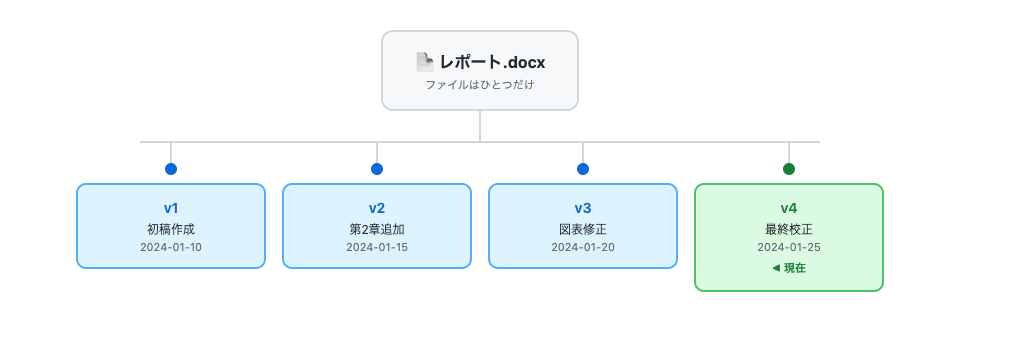
\includegraphics[width=0.9\textwidth]{images/diagram-version-tree.png}
\end{figure}

バージョン管理システムは、「いつ」「誰が」「何を」「なぜ」変更したのかを全て記録します。これにより、次のようなことが可能になります。

\begin{itemize}
  \item \textbf{過去の状態に戻る}: 3日前の状態に戻したい、というときにワンコマンドで実現できます
  \item \textbf{変更の追跡}: どの行がいつ変更されたかを正確に把握できます
  \item \textbf{並行作業}: 複数の人が同じプロジェクトで同時に作業しても、それぞれの変更を後から統合できます
  \item \textbf{バックアップ}: 変更履歴ごとデータが保存されるため、データの消失を防げます
\end{itemize}

\subsection{プログラミングにおけるバージョン管理}

プログラムのソースコードはテキストファイルであるため、バージョン管理との相性が抜群です。例えば、新しい機能を追加しようとしたがうまくいかなかった場合、バージョン管理があれば「機能追加前」の状態に簡単に戻せます。また、チーム開発では複数の開発者が同時にコードを書きますが、バージョン管理システムがそれぞれの変更を追跡し、矛盾なく統合してくれます。

現代のソフトウェア開発において、バージョン管理システムを使わずに開発するということは、まずありません。そして、今日世界で最も広く使われているバージョン管理システムが「Git」です。

\section{Gitとは}

\subsection{Gitの基本的な特徴}

Git（ギット）は、2005年にリーナス・トーバルズ（Linus Torvalds）によって開発された\textbf{分散型バージョン管理システム}です。リーナス・トーバルズは、世界で最も広く使われているオペレーティングシステムであるLinuxの作者としても知られています。

Gitの大きな特徴は「分散型」であるという点です。これは、プロジェクトの全ての変更履歴が各開発者のパソコンに完全にコピーされることを意味します。インターネットに接続していなくても、ローカル（自分のパソコン）だけで変更履歴の記録や確認ができるのです。

Gitは無料で使えるオープンソースソフトウェアであり、Windows、macOS、Linuxの全てで動作します。

\subsection{Gitが扱う基本概念}

Gitを理解するうえで欠かせない概念がいくつかあります。ここでは最も基本的なものを紹介します。それぞれの詳しい使い方は後続の章で改めて解説しますので、まずは「こういうものがあるのだな」という程度の理解で構いません。

\subsubsection{リポジトリ（Repository）}

リポジトリとは、プロジェクトのファイル群とその変更履歴の全てを格納する場所のことです。一般的には「リポ」や「repo（レポ）」と略されます。フォルダ（ディレクトリ）のようなものだと思ってください。

リポジトリには2種類あります。

\begin{itemize}
  \item \textbf{ローカルリポジトリ}: 自分のパソコン上にあるリポジトリ。日々の開発作業はここで行います。
  \item \textbf{リモートリポジトリ}: インターネット上のサーバー（GitHubなど）に置かれたリポジトリ。ローカルで行った変更をここに送信することで、他の開発者と共有できます。
\end{itemize}

\subsubsection{コミット（Commit）}

コミットとは、ある時点でのファイルの状態を履歴に記録する操作のことです。ゲームの「セーブポイント」に例えると分かりやすいでしょう。コミットを行うたびに、プロジェクトのスナップショット（その瞬間の状態）が保存されます。

\begin{lstlisting}[language={}]
コミット1 → コミット2 → コミット3 → コミット4（現在）
 "初期作成"   "機能A追加"  "バグ修正"   "機能B追加"
\end{lstlisting}

ひとつひとつのコミットには、次の情報が記録されます。

\begin{itemize}
  \item \textbf{誰が} 変更したか（Author）
  \item \textbf{いつ} 変更したか（Date）
  \item \textbf{何を} 変更したか（Diff: 変更差分）
  \item \textbf{なぜ} 変更したか（Commit Message: コミットメッセージ）
  \item \textbf{一意のID}（ハッシュ値: \cmd{a1b2c3d4e5f6...} のような文字列）
\end{itemize}

コミットメッセージは、将来の自分や他の開発者が「なぜこの変更を行ったのか」を理解するための手がかりになります。分かりやすいメッセージを書く習慣をつけることが大切です。

\subsubsection{ブランチ（Branch）}

ブランチは「枝」を意味する英語で、開発の流れを枝分かれさせる機能のことです。メインの開発ライン（多くの場合「main」というブランチ）に影響を与えることなく、新しい機能の開発やバグの修正を独立して進められます。

\begin{figure}[htbp]
\centering
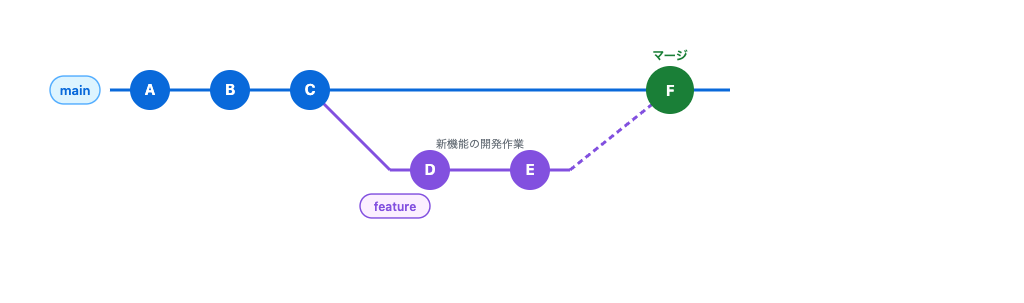
\includegraphics[width=0.9\textwidth]{images/diagram-branch-merge.png}
\end{figure}

この図では、mainブランチのCの時点で「feature」という新しいブランチが分岐しています。featureブランチでDとEという作業を行い、完成したらmainブランチに統合（マージ）しています。もしfeatureブランチでの作業がうまくいかなかったとしても、mainブランチには何の影響もありません。

\subsubsection{ステージング（Staging）}

ステージングとは、コミットに含めるファイルを選択する操作のことです。変更したファイルの全てをコミットするのではなく、「今回のコミットにはこのファイルとこのファイルだけを含める」といった選択ができます。

この仕組みは、変更を意味のあるまとまりに分けてコミットするために重要です。例えば、バグの修正と新機能の追加を同時に行った場合、ステージングを使えばそれぞれを別のコミットとして記録できます。

\begin{figure}[htbp]
\centering
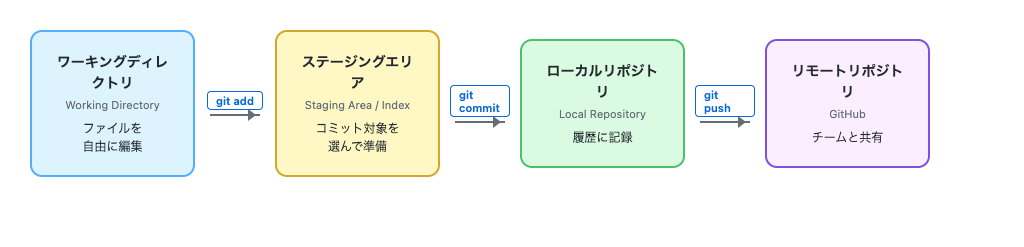
\includegraphics[width=0.9\textwidth]{images/diagram-staging.png}
\end{figure}

\section{GitHubとは}

\subsection{GitとGitHubの違い}

GitとGitHubは名前が似ていますが、全く別のものです。この違いを正しく理解することが非常に重要です。

\begin{table}[htbp]
\centering
\begin{tabular}{lll}
\hline
 & \textbf{Git} & \textbf{GitHub} \\
\hline
\textbf{正体} & バージョン管理ソフトウェア & Gitリポジトリのホスティングサービス \\
\textbf{動作する場所} & 自分のパソコン（ローカル） & インターネット上（クラウド） \\
\textbf{開発元} & Linus Torvalds（個人→コミュニティ） & GitHub社（現在はMicrosoft傘下） \\
\textbf{料金} & 完全無料 & 基本無料（有料プランあり） \\
\textbf{主な役割} & ファイルの変更履歴をローカルで管理する & Gitの履歴をオンラインで保存・共有する \\
\hline
\end{tabular}
\end{table}

Gitは自分のパソコンの中だけで動くソフトウェアです。一方、GitHubはGitで管理されたプロジェクトをインターネット上に保存し、他の人と共有するためのWebサービスです。

両者の関係は次の図のように表せます。

\begin{figure}[htbp]
\centering
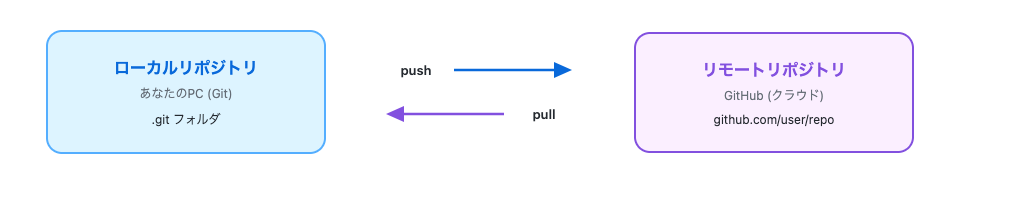
\includegraphics[width=0.9\textwidth]{images/diagram-push-pull.png}
\end{figure}

ローカルで行ったコミットを\cmd{push}（プッシュ）でGitHubに送信し、逆にGitHub上の変更を\cmd{pull}（プル）でローカルに取り込みます。この往復のやり取りによって、複数の開発者が同じプロジェクトを共有できるのです。

\subsection{GitHubが提供する付加価値}

GitHubは単なるGitリポジトリの保管場所ではありません。次のような豊富な機能を備えた開発プラットフォームです。

\begin{itemize}
  \item \textbf{プルリクエスト（Pull Request）}: コードの変更を提案し、レビューしてもらう仕組み
  \item \textbf{Issue}: バグ報告や機能要望を管理するチケットシステム
  \item \textbf{GitHub Actions}: テストやデプロイを自動化するCI/CD機能
  \item \textbf{GitHub Pages}: 静的Webサイトを無料でホスティング
  \item \textbf{Projects}: カンバンボードによるプロジェクト管理
\end{itemize}

これらの機能については第3部以降で詳しく解説します。

\section{Gitの歴史 — なぜGitは生まれたのか}

\subsection{Linuxカーネル開発とBitKeeper}

Gitが生まれた背景を理解するには、Linuxカーネルの開発史を知る必要があります。

Linuxカーネルは世界中の何千人もの開発者が参加する巨大なオープンソースプロジェクトです。2002年から2005年にかけて、このプロジェクトではBitKeeperという商用のバージョン管理ツールが無償で提供されており、開発者たちはそれを使ってコードを管理していました。

ところが2005年、BitKeeperの開発元がライセンスポリシーを変更し、無償利用ができなくなってしまいます。この出来事がGit誕生の直接のきっかけとなりました。

\subsection{10日間で作られたバージョン管理システム}

Linus Torvaldsは、既存のどのバージョン管理ツールもLinuxカーネルのような巨大プロジェクトには不十分だと考え、自分で新しいシステムを作ることを決意します。彼が掲げた設計目標は次のようなものでした。

\begin{itemize}
  \item \textbf{高速であること}: 何万ものファイルと長大な履歴を持つプロジェクトでも快適に動くこと
  \item \textbf{分散型であること}: 中央サーバーがなくても、各開発者のPCだけで完全に動作すること
  \item \textbf{データの完全性}: 一度記録した履歴が壊れたり改ざんされたりしないこと
  \item \textbf{非線形な開発への対応}: 何千ものブランチを同時に扱えること
\end{itemize}

驚くべきことに、Gitの最初のバージョンはわずか\textbf{10日間}で完成しました。2005年4月に開発が始まり、同年6月にはLinuxカーネルの管理がGitに移行されています。

「Git」という名前の由来について、Linus自身はユーモアを込めてこう語っています。「僕は自分のプロジェクトには自分にちなんだ名前を付けるんだ。最初がLinux、次がGitだ」。英語のスラングで「git」は「嫌なやつ」「ろくでなし」を意味する言葉で、自嘲的なネーミングです。一方で、"Global Information Tracker"（グローバル情報追跡装置）の頭文字だという解釈もあります。

\subsection{バージョン管理の進化の歴史}

Gitの革新性を理解するために、バージョン管理システムの歴史を振り返ってみましょう。

\begin{table}[htbp]
\centering
\begin{tabular}{lll}
\hline
\textbf{年代} & \textbf{システム} & \textbf{特徴} \\
\hline
1972年 & SCCS & 最初のバージョン管理システム。ファイル単位で管理 \\
1982年 & RCS & SCCSの改良版。依然としてファイル単位 \\
1990年 & CVS & ディレクトリ単位で管理可能に。中央集権型 \\
2000年 & Subversion（SVN） & CVSの後継。中央サーバーでの管理を洗練 \\
\textbf{2005年} & \textbf{Git} & \textbf{分散型。各PCに完全な履歴を保持。ここが大きな転換点} \\
\hline
\end{tabular}
\end{table}

2005年以前のバージョン管理システムは「中央集権型」と呼ばれ、変更履歴は中央のサーバーに一元管理されていました。開発者のパソコンには最新のファイルしかなく、履歴を確認したりブランチを切り替えたりするにはサーバーへの接続が必要でした。サーバーが故障すれば、全ての履歴が失われるリスクもありました。

Gitの「分散型」というアプローチでは、全ての開発者のパソコンにリポジトリの完全なコピー（全履歴を含む）が存在します。これにより、オフラインでも全ての操作が可能になり、サーバーが故障しても誰かのPCからデータを復元できるようになりました。

\begin{figure}[htbp]
\centering
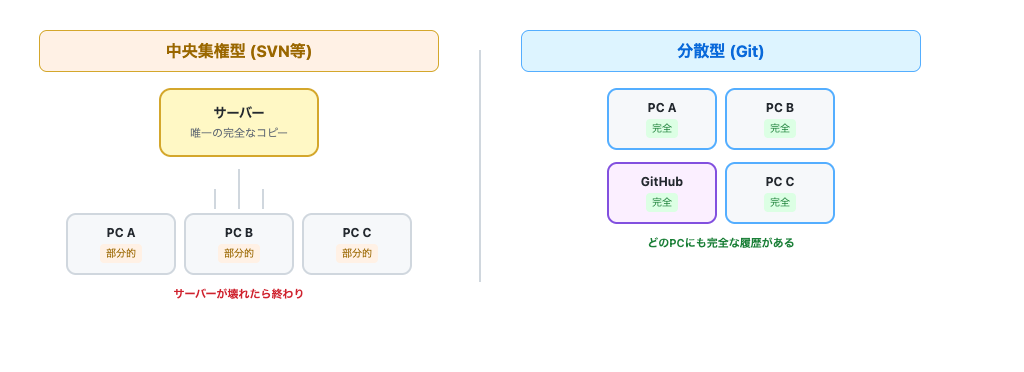
\includegraphics[width=0.9\textwidth]{images/diagram-centralized-vs-distributed.png}
\end{figure}

現在、Gitはバージョン管理システムの事実上の標準となっており、世界中の開発者の95\%以上がGitを使用していると言われています。

\section{GitHubの歴史 — ソフトウェア開発を変えた革命}

\subsection{GitHubの誕生と成長}

Gitは強力なバージョン管理ツールですが、コマンドラインでの操作が中心で、他の開発者との協業の仕組みはGit自体には含まれていませんでした。この課題を解決したのがGitHubです。

2008年2月、トム・プレストン=ワーナー（Tom Preston-Werner）、クリス・ワンストラス（Chris Wanstrath）、PJ・ハイエット（PJ Hyett）、スコット・チャコン（Scott Chacon）の4人がGitHubを設立し、サービスを公開しました。

以下はGitHubの歩みを示す年表です。

\begin{table}[htbp]
\centering
\begin{tabular}{lp{11cm}}
\hline
\textbf{年} & \textbf{出来事} \\
\hline
2008年 & GitHub設立・公開。公開1年で10万ユーザーを獲得 \\
2009年 & ホストするリポジトリが10万を突破 \\
2011年 & ユーザー数100万人を突破 \\
2012年 & 著名ベンチャーキャピタルのAndreessen Horowitzから1億ドル（約130億円）の資金調達 \\
2013年 & リポジトリ数が1,000万を突破 \\
2018年 & Microsoftが75億ドル（約1兆円）でGitHubを買収。当初は懸念の声もあったが、GitHubの独立性は維持された \\
2019年 & GitHub Actions（CI/CD機能）リリース。プライベートリポジトリが無料プランでも利用可能に \\
2020年 & npm（Node.jsのパッケージ管理システム）を買収。ユーザー数5,600万人 \\
2021年 & GitHub Copilot（AIコーディング支援）のプレビューを開始 \\
2022年 & GitHub Copilotを一般公開 \\
2023年 & ユーザー数1億人を突破。リポジトリ数は3億7,200万超 \\
2024年 & Copilot Workspace、GitHub Modelsなど、AIを活用した新機能を次々と発表 \\
2025年 & ユーザー数1億5,000万人を超え、世界最大の開発プラットフォームとして不動の地位を確立 \\
\hline
\end{tabular}
\end{table}

\subsection{GitHubが世界にもたらした変革}

GitHubは単にGitリポジトリをホストするサービスを超えて、ソフトウェア開発の文化そのものを変革しました。

\subsubsection{オープンソースの民主化}

GitHub以前の時代、オープンソースソフトウェア（OSS）に貢献するのは敷居の高い行為でした。プロジェクトのメーリングリストを見つけ、パッチファイルを作成し、メールで送信し、メンテナの返事を待つ——こうした手順は、経験の浅い開発者にとって大きな壁でした。

GitHubは「Fork（フォーク）」と「Pull Request（プルリクエスト）」という仕組みを洗練させることで、この壁を取り払いました。気になるプロジェクトを見つけたら、ボタンひとつで自分のアカウントにコピーし、修正を加え、元のプロジェクトに提案する——このシンプルな流れが、世界中の何百万人もの開発者がOSSに貢献するきっかけを作りました。

\subsubsection{ソーシャルコーディングの概念}

GitHubは開発者のための「SNS」としての側面も持っています。他の開発者をフォローしたり、気に入ったリポジトリにスター（星マーク）を付けたり、コントリビューショングラフ（通称「草」と呼ばれる、1年間の活動量を緑色の濃淡で表示する図）で日々の活動を可視化したり——こうした機能が開発者同士のつながりを促進しています。

\subsubsection{世界を動かすプロジェクトの集積地}

今日、世界を動かす多くのソフトウェアがGitHub上でホストされています。

\begin{table}[htbp]
\centering
\begin{tabular}{lp{10cm}}
\hline
\textbf{プロジェクト} & \textbf{説明} \\
\hline
\textbf{Linux} & 世界のサーバーの大半、Androidの基盤となるOSカーネル \\
\textbf{React} & Meta社（旧Facebook）が開発したWebフロントエンドライブラリ \\
\textbf{VS Code} & Microsoft製のソースコードエディタ \\
\textbf{TensorFlow} & Google製の機械学習フレームワーク \\
\textbf{Python (CPython)} & Python言語の公式実装 \\
\textbf{Kubernetes} & コンテナ化されたアプリケーションの運用管理ツール \\
\hline
\end{tabular}
\end{table}

これらのプロジェクトは全てオープンソースとしてGitHub上に公開されており、世界中の開発者がコードを読み、バグを報告し、改善を提案しています。

\subsubsection{開発者の「履歴書」としてのGitHub}

技術者の採用面接において、GitHubアカウントが「技術力の証明」として活用されるようになりました。どんなプロジェクトに貢献しているか、どの程度の頻度でコードを書いているか、コードの品質はどうか——GitHubのプロフィールページがこれらを雄弁に語ってくれます。

\subsection{GitHubの競合サービス}

GitHubが圧倒的なシェア（推定90\%以上）を持つ一方で、他にもGitリポジトリのホスティングサービスは存在します。

\begin{table}[htbp]
\centering
\begin{tabular}{lp{10cm}}
\hline
\textbf{サービス} & \textbf{特徴} \\
\hline
\textbf{GitLab} & セルフホスト（自社サーバーでの運用）が可能。CI/CD機能が充実。DevOps全般をカバー \\
\textbf{Bitbucket} & Atlassian社製。同社のJira（プロジェクト管理）やConfluence（ドキュメント）と密に連携 \\
\textbf{Gitea} & 軽量なセルフホスト型。Go言語で書かれており、小規模チーム向け \\
\textbf{Azure DevOps} & Microsoft製のエンタープライズ向け開発プラットフォーム \\
\hline
\end{tabular}
\end{table}

組織のセキュリティポリシーや既存のツール群との相性によって、GitLab やBitbucketが選ばれるケースもありますが、本書ではGitHubの使い方に焦点を当てて解説していきます。

\section{Git/GitHubを使うメリット}

ここまでの内容を踏まえて、Git/GitHubを使うことのメリットを整理しましょう。

\begin{enumerate}
  \item \textbf{変更履歴が全て残る} — いつでも過去の状態に戻れるため、「あの変更を元に戻したい」という場面で困ることがありません。
  \item \textbf{複数人で同時作業できる} — ブランチを使って独立した作業を進め、後から統合できます。同じファイルを複数人が触ったとしても、Gitが変更点を追跡してくれます。
  \item \textbf{バックアップになる} — GitHubにコードが保存されるため、パソコンが壊れてもプロジェクトを失うことがありません。
  \item \textbf{コードレビューができる} — プルリクエストを通じて、他の人にコードを読んでもらい、改善点を指摘してもらえます。
  \item \textbf{オープンソースへの参加} — 世界中の優れたプロジェクトのコードを読み、学び、貢献することができます。
  \item \textbf{ポートフォリオとして活用} — GitHubのプロフィールとリポジトリが、あなたの技術力を示すポートフォリオになります。
\end{enumerate}

\section{まとめ}

本章では、以下の内容を学びました。

\begin{itemize}
  \item \textbf{バージョン管理}とは、ファイルの変更履歴を体系的に記録・管理する仕組みのことである
  \item \textbf{Git}はローカルで動作する分散型バージョン管理ソフトウェアであり、\textbf{GitHub}はGitリポジトリをオンラインでホスティングするサービスである。両者は補完関係にある
  \item Gitの基本概念として、\textbf{リポジトリ}（プロジェクトの器）、\textbf{コミット}（変更の記録）、\textbf{ブランチ}（開発の分岐）、\textbf{ステージング}（コミット対象の選択）がある
  \item Gitは2005年にLinuxカーネルの管理のために生まれ、GitHubは2008年の設立以来、オープンソースの民主化やソーシャルコーディングの概念を通じてソフトウェア開発の世界を大きく変えた
\end{itemize}

次の章では、実際にGitを自分のパソコンにインストールする手順を見ていきます。
